\section{L'azienda}
{\company} è un'azienda con quarant'anni di esperienza nell'offrire a piccole e medie imprese soluzioni informatiche per la 
gestione e l'automazione dei processi aziendali. I suoi prodotti di punta sono infatti sistemi \gls{erp} (\textit{Enterprise 
Resource Planning}) ovvero sistemi che permettono di coordinare il flusso di dati tra i processi di un'azienda, fornendo un'unica fonte di 
informazioni e semplificandone le operazioni.\\
{\company} è situata a Pernumia (Padova) e opera in prevalenza nel Nord Est, dal 2016 è entrata a far parte del gruppo Officegroup, azienda 
che riunisce diverse \textit{software house} specializzate nella progettazione e sviluppo di sistemi gestionali evoluti. 
Dal 2023 inoltre è diventata una società \textit{benefit}, ovvero è un azienda che opera con l'obiettivo di generare un impatto positivo 
sulla società e sull'ambiente, oltre al profitto finanziario.

\begin{figure}[H]
    \centering
    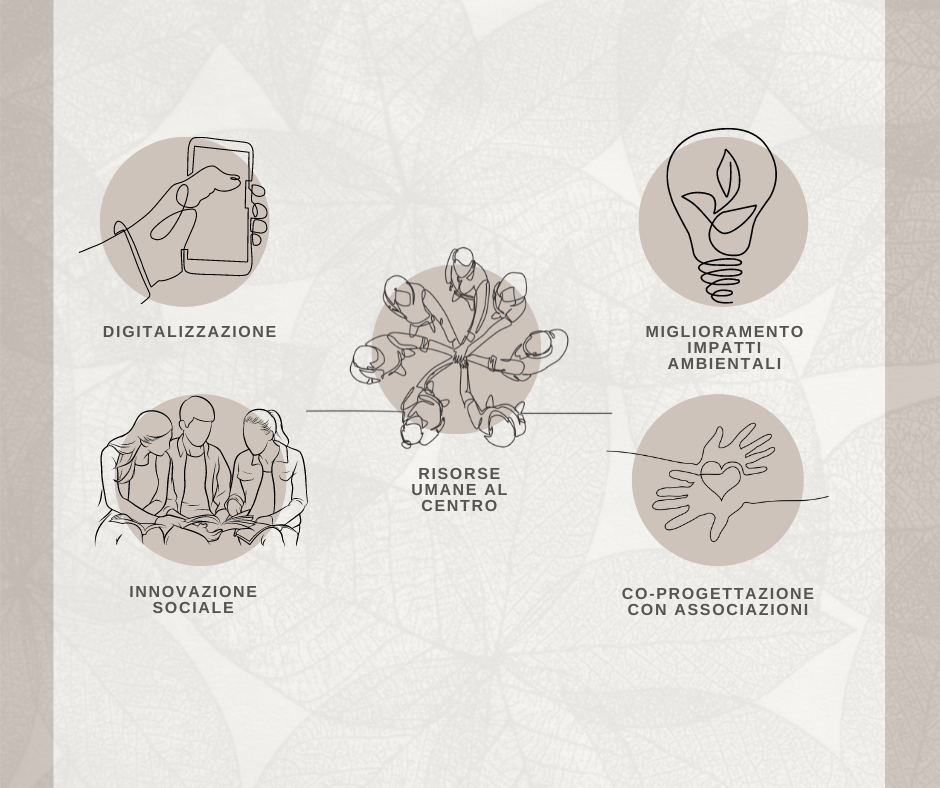
\includegraphics[alt={Obbiettivi delle società benefit}, width=0.5\textwidth]{img/soc-benefit.png}
    \caption{Obbiettivi delle società benefit. \\ \textit{fonte: https://www.vsh.it/azienda/societa-benefit/}}
    \label{fig:società benefit}
\end{figure}

Come mostrato in Figura \ref{fig:società benefit} questo tipo di società attuano iniziative in diversi ambiti, dalla dematerializzazione 
e digitalizzazione alla promozione di politiche a sostegno della conciliazione vita-lavoro.\\
Altri obbiettivi delle società \textit{benefit} possono essere: investire nelle energie rinnovabili e la sostenibilità, l'investimento in tecnologie 
ad alta efficienza energetica, rispetto della parità di genere, formazione professionale del lavoratore, progetti con scuole ed 
università, co-progettazione con associazioni e istituzioni del territorio con il duplice obiettivo di stimolare la partecipazione dei dipendenti 
a “buone cause” della comunità e valorizzare il lavoro di associazioni no-profit del territorio, generando così valore sociale.

